	Son aquellos que trabajan por cargas, es decir se introduce una alimentación, y se espera un tiempo dado, que viene determinado por la cinética de la reacción, tras el cual se saca el producto.
	
	\section{Reactor discontinuo isotermo}
	A partir del balance de materia se obtiene la ecuación que proporciona el tiempo de reacción a partir de la velocidad de reacción en este modo de operación es:
	
	\begin{equation*}
	t = C_{A0}\int_{X_{A0}}^{X_A}\frac{dX_A}{(-r_a)}
	\end{equation*}
	
	Donde $(-r_a)$ se puede calcular como:
	
	\begin{equation*}
	(-r_a) = K \cdot C_{A0}^n (1-X_A)^n; ~~~~~ K = K_0\exp\left(\frac{-E_a}{RT}\right)
	\end{equation*}
	
	Según el orden de reacción el tiempo se podrá calcular como:
	
	\begin{itemize}
		\item Orden 0: $ t = \frac{C_{A0}}{K}(X_A-X_{A0})$
		\item Orden 1: $ t = \frac{1}{K}\ln\left(\frac{1-X_{A0}}{1-X_A}\right)$
		\item Orden 2: $ t = \frac{1}{KC_{A0}}\left(\frac{X_A}{1- X_A}\right)$
	\end{itemize}
	
	En la Figura \ref{dis_iso} se puede ver la pantalla para definir los parámetros del reactor que son: 
	\begin{itemize}
		\item Orden de reacción.
		\item Temperatura inicial [K].
		\item Concentración inicial [mol/l].
		\item Energía de activación [J/mol].
		\item Constante $k_0$.
		\item Conversión inicial y final.
	\end{itemize}
	\begin{figure}[!h]
		\centering
		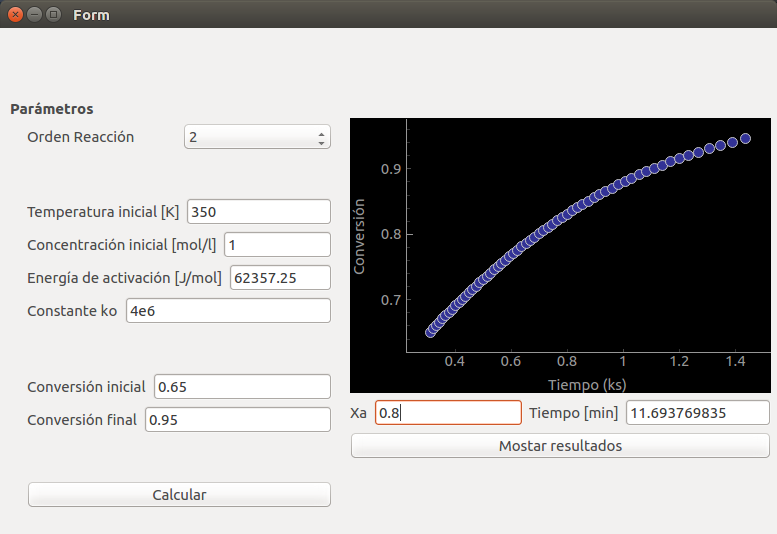
\includegraphics[width=0.9\textwidth]{./imagenes/reactor_discontinuo/Form_048.png}
		\label{dis_iso}
		\caption{Ventana de cálculo del reactor discontinuo e isotermo.}
	\end{figure}

	La aplicación tiene un cuadro de texto donde se puede introducir una conversión y automáticamente se rellena el campo que se encuentra al lado con el tiempo en  minutos que se tarda en alcanzar esa conversión. Todos los reactores cuentan también con esta característica.
	
	Todas las ventanas también cuentan con un botón que pone ``Mostrar resultados'' este botón genera una nueva ventana donde se puede ver la misma gráfica con un cursor para poder ver los datos de la curva. Esta ventana también permite guardar la gráfica. En la Figura \ref{dis_iso_graf} se puede ve la ventana generada con el botón ``Mostrar resultados''.
	
	\begin{figure}[!h]
		\centering
		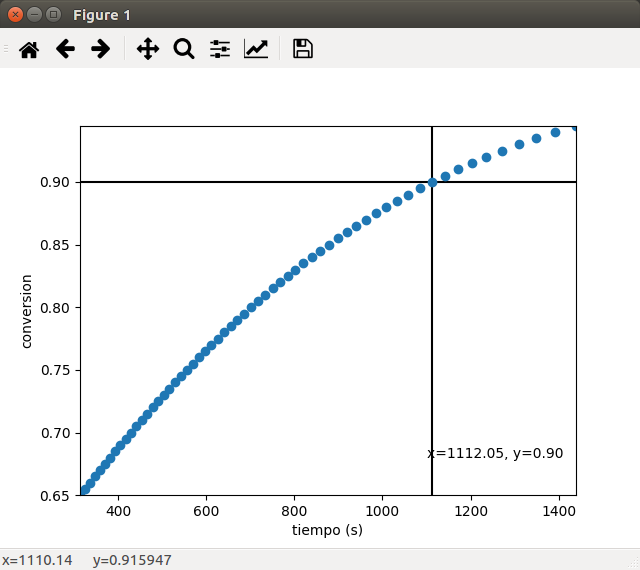
\includegraphics[width=0.9\textwidth]{./imagenes/reactor_discontinuo/iso_fig.png}
		\label{dis_iso_graf}
		\caption{Ventana con el resultado de un reactor isotermo.}
	\end{figure}
	
	\section{Reactor discontinuo adiabático}
	La ecuación que proporciona el tiempo de reacción en este modo de operación es:
	
	A partir del balance de materia se obtiene:
	\begin{equation*}
	t = C_{A0}\int_{X_{A0}}^{X_A}\frac{dX_A}{(-r_a)}
	\end{equation*}
	
	Donde $(-r_a)$ se puede calcular como:
	
	\begin{equation*}
	(-r_a) = K \cdot C_{A0}^n (1-X_A)^n; ~~~~~ K = K_0\exp\left(\frac{-E_a}{RT}\right)
	\end{equation*}
	
	A partir del balance de energía se obtiene:
	\begin{equation*}
	T = T_0 + \frac{(-\Delta H_R)C_{A0}}{\rho C_p}(X_A-X_{A0})
	\end{equation*}
	
	Los parámetros necesarios para el diseño del reactor son:
	
	\begin{itemize}
		\item Orden de reacción.
		\item Temperatura inicial [K].
		\item Concentración inicial [mol/l].
		\item Energía de activación [J/mol].
		\item Constante $k_0$.
		\item Calor de reacción [J/mol].
		\item Peso molecular [g/mol].
		\item Calor específico [J/(kg·K)].
		\item Densidad de la mezcla [kg/m3].
		\item Tipo de reacción (exotérmica, endotérmica).
		\item Conversión inicial y final.
	\end{itemize}

	En la Figura \ref{dis_adi} se puede ver la ventana para el cálculo de un reactor discontinuo y adiabático.
	
	\begin{figure}[!h]
		\centering
		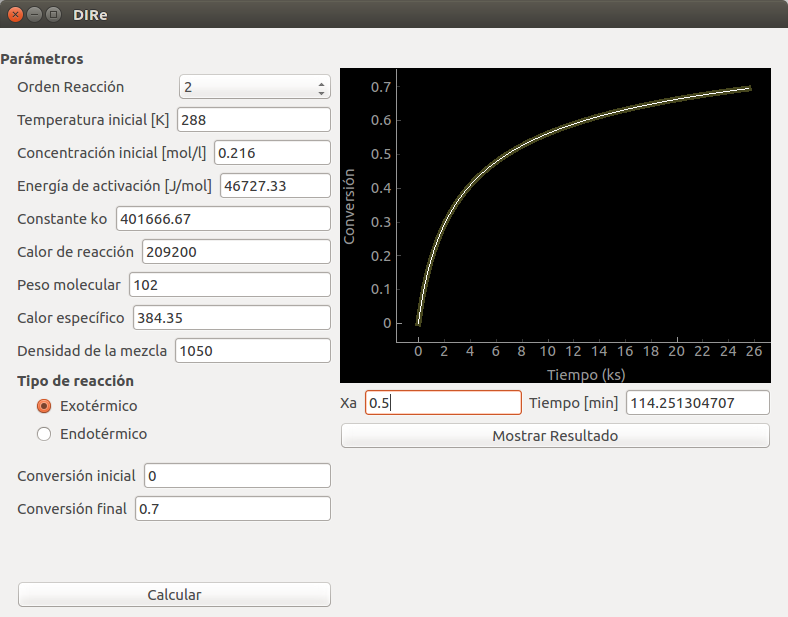
\includegraphics[width=0.9\textwidth]{./imagenes/reactor_discontinuo/adi.png}
		\label{dis_adi}
		\caption{Ventana de cálculo del reactor discontinuo y adiabático.}
	\end{figure}

	\section{Reactor discontinuo no discontinuo y no adiabático}
	La ecuación que proporciona el tiempo de reacción en este modo de operación es:
	
	A partir del balance de materia se obtiene:
	\begin{equation*}
	\frac{dt}{dX_A} = \frac{C_{A0}}{K_0 \exp\left(\frac{-E}{RT}\right) C_{A0}^n (1-X_A)^n}
	\end{equation*}
	
	A partir del balance de energía se obtiene:
	\begin{equation*}
	\frac{dT}{dX_A} = \frac{(-\Delta H_R)C_{A0}}{\rho C_p} + \frac{C_{A0}US(T_c-T)}{V\rho C_p K_0 \exp\left(\frac{-E_a}{RT}\right)C_{A0}^n(1-X_A)^n}
	\end{equation*}
	
	Los parámetros necesarios para el diseño del reactor son:
	
	\begin{itemize}
		\item Orden de reacción.
		\item Temperatura inicial [K].
		\item Concentración inicial [mol/l].
		\item Energía de activación [J/mol].
		\item Constante $k_0$.
		\item Calor de reacción [J/mol].
		\item Peso molecular [g/mol].
		\item Calor específico [J/(kg·K)].
		\item Densidad de la mezcla [kg/m3].
		\item Coeficiente de transmisión de calor [W/(m·K)].
		\item Área de transmisión de calor [m2].
		\item Volumen [m3]. 
		\item Tipo de reacción (exotérmica, endotérmica).
		\item Conversión inicial y final.
	\end{itemize}
	
	En la Figura \ref{dis_no_iso_no_adi} se puede ver la ventana para el cálculo de un reactor discontinuo que no es isotermo ni adiabático.
	\begin{figure}[!h]
		\centering
		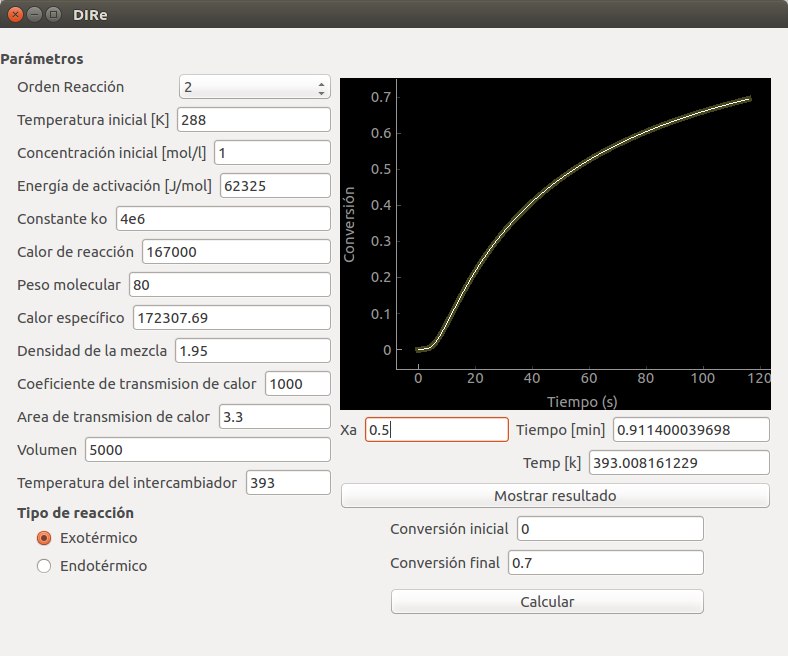
\includegraphics[width=0.9\textwidth]{./imagenes/reactor_discontinuo/no_iso_no_adi.png}
		\label{dis_no_iso_no_adi}
		\caption{Ventana de cálculo del reactor discontinuo que no es isotermo ni adiabático.}
	\end{figure}

	
	En este tipo de reactor cuando se pulsa el botón de ``Mostrar resultados'' se muestran dos gráficas, una de ellas muestra la conversión frente al tiempo y la otra la temperatura frente al tiempo. Ver Figura \ref{dis_no_iso_no_adi_fig}.
	
	\begin{figure}[!h]
		\centering
		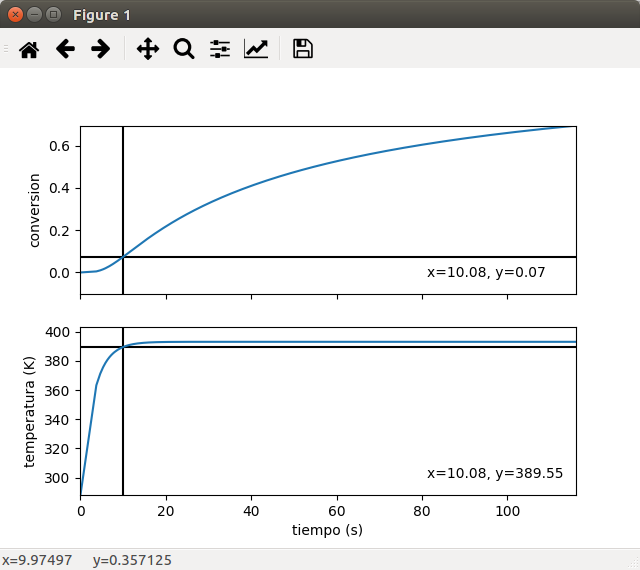
\includegraphics[width=0.8\textwidth]{./imagenes/reactor_discontinuo/no_iso_no_adi_fig.png}
		\label{dis_no_iso_no_adi_fig}
		\caption{Resultado del cálculo del reactor discontinuo que no es isotermo ni adiabático.}
	\end{figure}